\documentclass{emulateapj}

\usepackage{epsfig}
\usepackage{amsmath}
\usepackage{rotating}
\usepackage{natbib}
%\usepackage{lscape}
\usepackage{enumerate}
\usepackage{multirow}
\usepackage{array}
\usepackage{appendix}
\usepackage{comment}
\usepackage{color}
%\usepackage[dvipdfmx]{color}
%\usepackage[dvipdfmx]{graphicx}

\bibliographystyle{apj}

\def\memoYF#1{\color{red}$[${\bf #1}$]$ \color{black}}

\def\memoDS#1{\color{blue}$[${\bf #1}$]$ \color{black}}

\def\plotonesc#1{\centering \leavevmode
\includegraphics[clip=, width=1.70\columnwidth]{#1}}
\def\plotoneh#1{\centering \leavevmode
\includegraphics[clip=, width=.95\columnwidth]{#1}}
\def\plotone#1{\centering \leavevmode
\includegraphics[clip=, width=.85\columnwidth]{#1}}
\def\plotoneShrinkSmall#1{\centering \leavevmode
\includegraphics[clip=, width=.49\columnwidth]{#1}}
\def\plotoneShrinkMed#1{\centering \leavevmode
\includegraphics[clip=, width=.55\columnwidth]{#1}}
\def\plotoneShrinkBig#1{\centering \leavevmode
\includegraphics[clip=, width=.65\columnwidth]{#1}}
\def\plottwo#1#2{\centering \leavevmode
\includegraphics[width=.45\columnwidth]{#1} \hfil
\includegraphics[width=.45\columnwidth]{#2}}
\def\plottwob#1#2{\centering \leavevmode
\includegraphics[width=.49\columnwidth]{#1} \hfil
\includegraphics[width=.49\columnwidth]{#2}}
\def\plottwor#1#2{\centering \leavevmode
\includegraphics[width=.55\columnwidth,angle=90]{#1} \hfil
\includegraphics[width=.55\columnwidth,angle=90]{#2}}
\def\plotthree#1#2#3{\centering \leavevmode
\includegraphics[width=.3\columnwidth]{#1} \hfil
\includegraphics[width=.3\columnwidth]{#2} \hfil
\includegraphics[width=.3\columnwidth]{#3}}

\newcommand{\cN}[1]{\mathcal{N}}
\newcommand{\pn}[1]{\mbox{$(#1)$}}
\newcommand{\spa}{\mbox{ }}
\def\gsim{\;\rlap{\lower 2.5pt
 \hbox{$\sim$}}\raise 1.5pt\hbox{$>$}\;}
\def\lsim{\;\rlap{\lower 2.5pt
   \hbox{$\sim$}}\raise 1.5pt\hbox{$<$}\;}

% set formatting properties
\setlength{\textwidth}{6.5in}
\setlength{\textheight}{8.8in}
\setlength{\hoffset}{0.0in}
\setlength{\voffset}{-0.4in}
%\setlength{\voffset}{0.3in}
\parindent 0.2in
\parskip 0.1in



%%%%%%%%%%%%%%%%%%%%%%%%%%%%%%%%%%%%%%%%%%%%%%%%%
% THE DOCUMENT BEGINS HERE                      %
%%%%%%%%%%%%%%%%%%%%%%%%%%%%%%%%%%%%%%%%%%%%%%%%%

%\slugcomment{Submitted to ApJ, 20 October 2011}

\begin{document}


%%% Begin front material
%\twocolumn[%%% Begin front material

\title{Red-Giant Hot Jupiters: Brilliant Radio Beacons?}

\author{
%
Yuka Fujii\altaffilmark{0} \\
%
David S. Spiegel\altaffilmark{1, 2} \\
%
{\bf and some order:} \\
%
Jason Nordhaus\altaffilmark{3} \\
%
Nikku Madhusudhan\altaffilmark{4} \\
%
Mehrdad Mirbabayi\altaffilmark{1} \\
%
Aaron Parsons\altaffilmark{5} \\
%
Tony Mroczkowski\altaffilmark{6} \\
%
Neil Zimmerman\altaffilmark{7}
}

\affil{$^0$Earth-Life Science Institute, Tokyo Institute of Technology, 
  Tokyo, JAPAN, 152-8550}
  
\affil{$^1$Astrophysics Department, Institute for Advanced Study,
  Princeton, NJ 08540}

\affil{$^2$Research \& Development, Sum Labs,
  New York, NY  10001}

\affil{$^2$Department of Mathematics, Rochester Institute of Technology}

\affil{$^3$Astronomy Department, University of Cambridge, UK}

\affil{$^4$Astronomy Department, UC Berkeley}

\affil{$^5$Naval Research Laboratory}

\affil{$^6$Department of Mechanical and Aerospace Engineering, Princeton University, Princeton, NJ 08544}


\vspace{0.5\baselineskip}

\email{
dave@ias.edu
}


\begin{abstract}
  Red-giant hot Jupiters are jovian planets orbiting red-giant-branch
  or asymptotic-giant-branch (AGB) stars.  Post-main-sequence stars
  lose mass at much higher rates than main-sequence stars.  A jovian
  planet passing through the dense winds of its AGB host can capture
  stellar wind in its magnetosphere.  The cyclotron frequency of
  electrons from the stellar wind accreting onto the planet scales as
  100~MHz~$(B/30 {\rm~Gauss})$.  Such a planet might generate a radio
  luminosity that would be visible from kiloparsec distances.
\end{abstract}


\keywords{planets and satellites: Jupiter --- Sun: evolution ---
  planetary systems --- radiative transfer --- stars: evolution ---
  stars: AGB and post-AGB}
%]%%% End front material

%%%%%%%%%%%%%%%%%%%%%%%%%%%%%%%%%%%%%%%%%%%%%%%%%%%%%%%%%%%%%%%%%%%
\section{Introduction}
\label{sec:intro}
%%%%%%%%%%%%%%%%%%%%%%%%%%%%%%%%%%%%%%%%%%%%%%%%%%%%%%%%%%%%%%%%%%%



Planets with strong magnetic fields may generate radio or X-ray emission when interacting with energetic charged particles. 
It has been known that Jupiter emits radio emission from the radiation belt and auroral region due to the acceleration of the plasmas. \memoYF{?}. Potentially, large exoplanets can also emit radio waves through the similar mechanisms, depending on their intrinsic magnetic fields and the density of surrounding plasmas, e.g. stellar wind particles and particles from Io-like moons. 
Radio emissions from exoplanets have been estimated taking account of several possible processes, based on the empirical scaling of the radio intensity with the solar wind flux \citep{zarka2001,griebmeier2007,noyola2014}. 
Although the search for these radio signatures are being conducted, there is no clear detection claimed so far, while some indications were obtained \memoYF{?} \citep{lecavelier_et_al2013}. 
%In general, there are four proposed models for a planet to emit radio wave \citep{griebmeier2007}: 1) the magnetic energy model, 2) kinetic energy model, 3) CME model, and 4) the unipolar interaction model. 
%The search for these radio emissions from extrasolar Jovian planets has been performed. 


%It has been predicted that
% fix
When stars less than $\sim$8~$M_\sun$ evolve off the main sequence,
they go through stages on the red-giant branch (RGB) and the
asymptotic-giant branch (AGB) where their radii and luminosities increase by orders of magnitude. 
Jovian planets in orbit around such stars can be transiently heated to hot-Jupiter temperatures ($\sim$1000~K or more) at distances out to tens of AU, depending on the star's mass \citep{spiegel+madhusudhan2012}. 
At the same time, they are subject to massive (but slow) stellar wind, as the mass-loss rate of such evolved stars are significantly higher than the main-sequence counterparts, typically $\sim  10^{-8} M_{\odot }$/yr \citep{judge1991}. 
The mass-loss rate can be as high as $\sim  10^{-5} M_{\odot }$/yr for AGB stars. 
\memoYF{to Jason: how these values are observationally obtained? Suggestions for relevant references?} 
%stellar wind \citep{suzuki2008} \memoYF{To Jason: references?}. 
On the assumption that the radio emission is correlated with the stellar wind, planetary companions around evolved stars could generate bright radio emission. 

In this paper we estimate the potential to detect planetary companions around evolved stars through the brightness of their radio emission. 
%The search for such emission could tell us the population of companions around evolved stars, including those were originally A or O stars. 
In \S2, we describe our assumptions for the scaling of planetary radio emission, stellar wind, and planetary magnetosphere.  
\S3 estimates spectral radio intensity from RGHJs and compare them that from canonical hot Jupiters. 
\S4 discusses possible obstacles to detect radio emission from RGHJs, in particular the effects of intrinsic radio emission of evolved stars and the  offsetting effect of the electrons spiraling down along the planetary magnetic field. Observability with current and near-future instruments is also examined in \S4. 
Finally, \S5 concludes the paper with a brief summary. 
% based on the number of targets in the observable volumes


%Red giants lose their masses at a high rate, typically $\sim  10^{-5} M_{\odot }/yr $ through massive stellar wind. These stellar wind particle can 


%Roughly 20\% of the more than 700 \memoYF{check!} currently known exoplanets around main-sequence stars \footnote{See online catalogs such as http://www.openexoplanetcatalogue.com/ \citep{rein2012}, http://exoplanet.eu \citep{schneider_et_al2011}, or http://exoplanets.org \citep{wright_et_al2011} for up-to-date lists.} have masses greater than half of Jupiter's, orbital radii greater than 1~AU, and will become hot Jupiters (i.e., for the present purposes, this means they will receive at least as much irradiation as the currently known hot Jupiters/Neptunes \citep{spiegel+madhusudhan2012}. 


%%%%%%%%%%%%%%%%%%%%%%%%%%%%%%%%%%%%%%%%%%%%%%%%%%%%%%%%%%%%%%%%%%%
\section{Model}
\label{s:assumptions}
%%%%%%%%%%%%%%%%%%%%%%%%%%%%%%%%%%%%%%%%%%%%%%%%%%%%%%%%%%%%%%%%%%%


Before estimating the frequency of planetary radio emission and the spectral radio intensity, we specify the property of the stellar wind of the evolved stars in \S\ref{ss:stellarwind}, and that of planetary magnetic field in \S\ref{ss:magneticfield}.  
Then, we discuss the framework to estimate the frequency and intensity of planetary radio emission in \S\ref{ss:model_frequency} and \S\ref{ss:model_intensity}, respectively. 



%%%%%%%%%%%%%%%%%%%%%%%%%%%%%%%%%%%%%%%%%%%%%%%%%%%%%%%%%%%%%%%%%%%
\subsection{Assumptions for Stellar Wind}
\label{ss:stellarwind}
%%%%%%%%%%%%%%%%%%%%%%%%%%%%%%%%%%%%%%%%%%%%%%%%%%%%%%%%%%%%%%%%%%%

One important factor in modeling the radio emission due to the interaction with stellar wind and the planetary magnetic field is the density and velocity of stellar wind. 
The number density of stellar wind, $n$, can be expressed as
%%%
\begin{equation}
n = \frac{\dot M}{4\pi a^2 m_p v}
\end{equation}
%%%
where $\dot M$ is the mass loss rate, $a$ is the orbital distance from the star and $m_p$ is proton mass, and $v$ is the velocity of the stellar wind. 

While the solar mass loss rate, $\dot M_{\odot }$, is $\dot M_{\odot } \sim 2\times 10^{-14} M_{\odot}$/yr \memoYF{reference needed?}, the mass loss rate of red giants is significantly greater, typically $\dot M \sim 10^{-8} M_{\odot}$/yr based on observation \memoYF{to Jason: reference?}. The rate can be as high as $10^{-5} M_\odot{\rm /yr}$ during the AGB phase. 
Therefore, we have
%\memoDS{Can be as high as $10^{-5} M_\odot~{\rm yr^{-1}}$ during AGB phases.  I'm calling it ``red giant'' but we're really thinking of AGB stars for maximum mass-loss and brightness.}
\begin{equation}
\frac{\dot M}{\dot M_{\odot}} \sim 10^6 - 10^9
\end{equation}

On the other hand, the stellar wind velocity becomes smaller because of the small escape velocity (due to expanded stellar radius).
%\footnote{Escape velocity is $\sqrt{2GM/r}$.}
Assuming that the stellar wind scales as the escape velocity, i.e., $\propto \sqrt{2GM_p/R}$ ($G$ is the gravitational constant, $M_p$ is the planetary mass, and $R$ is the planetary radius), a RG with radius $R=100R_{\odot}$ has 10 times as slow stellar wind as that at the main sequence. \memoYF{Estimate in more detail?} Thus, 
\begin{equation}
\frac{v}{v_{\odot}} \sim 10^{-1}
\end{equation}
where $v_{\odot} \sim 4.0 \times 10^5 $ km/sec. 

%The temperature of stellar wind of RGs is expected to be 2 orders of magnitude lower than their main sequence counterparts, mainly because the sound speed of hot corona exceeds the escape speed, i.e., hot corona cannot be confined in the stellar atmosphere \citep{suzuki2008}. 
%\begin{equation}
%\frac{T}{T_{\odot}} \sim 10^{-2}
%\end{equation}
%where $T_{\odot } \sim 10^6$ K. 

%%%%%%%%%%%%%%%%%%%%%%%%%%%%%%%%%%%%%%%%%%%%%%%%%%%%%%%%%%%%%%%%%%%
\subsection{Assumptions for Planetary Magnetic Field}
\label{ss:magneticfield}
%%%%%%%%%%%%%%%%%%%%%%%%%%%%%%%%%%%%%%%%%%%%%%%%%%%%%%%%%%%%%%%%%%%

In order to estimate the planetary magnetic field of general planets, we adopt a simple scaling relation between the magnetic field and macroscopic planetary properties. 

Several relationships have been proposed so far \citep[e.g.][]{russel1978,busse1976,stevenson1979,mizutani1992,sano1993,starchenko2002,christensen2006} \memoYF{check!} (see \citet{griebmeier2004} or \citet{christensen2010} for the summary). 
%
They are compared with numerical simulations in \citet{christensen2010}. We employ the following relationship from \citet{christensen2006}, which was found to be in a good agreement with the numerical experiments over a wide parameter space \memoYF{describe in more detail}:
%%%%%%%%%% 
\begin{equation}
B^2 \propto \rho_c r_c^{4/3} q_c^{2/3}, \label{eq:Bscaling} % \omega ^{\alpha } \rho_c ^{\beta } r_c^{\gamma } \sigma ^{\delta } 
\end{equation}
%%%%%%%%%%
where $\rho _c$ and $r_c$ are the density and the radius of the dynamo region, and $q_c$ is the internal convected energy flux in the core region. 

In order to evaluate $\rho _c $ and $r_c$, we need a model of internal structure of planets. 
In this paper, we consider Jupiter-like gaseous planets and assume that the planetary radius is constant at $R_p = R_{p,J}$, because the numerical calculations show that the radii of gaseous planets over the range of $0.1 M_{p, J} < M_p < 10M_{p, J}$ (with core mass less than 10\%) are converged to $0.8 R_{p, J} < R_p < 1.2R_{p, J}$ within 1 Gyr \citep{fortney2007}. 
For the density profile, we assume a polytrope gas sphere with index $n=1$, which results in:
%%%%%%%%%% 
\begin{equation}
\rho [r] = \left( \frac{\pi M_p}{4 R_p^3} \right) \frac{\sin \left[ \pi \frac{r}{R_p} \right]}{\left( \pi \frac{r}{R_p} \right)}. \label{eq:rho_r}
\end{equation}
%%%%%%%%%%
We determine the core radius $r_c$ by assuming that the hydrogen becomes metallic when $\rho (r)$ exceeds the critical density $\rho_{\rm crit}=700\,\mbox{kg/m}^3$ \memoYF{cite something!}. The density of the metallic core, $\rho _c$ is obtained by averaging the density in the core. 
In the case of Jupiter, $r_{c,\,J} = 0.85 R_{\rm J}$. 
%We assume that the conductivity $\sigma $ is the same as Jupiter \memoYF{?}. 

The convected heat flux, $q_c$, is estimated by dividing the time-dependent net planetary luminosity by the surface area of the core region ($4\pi r_c^2$). 
The model of luminosity evolution is taken from \citet{burrows_et_al2001} \citep[see also][]{marley2007}, which resulted in:
%%%%%%%%%%
\begin{equation}
L \sim {10^{-8} L_\odot} \left( \frac{t}{1 \rm~Gyr} \right)^{-1.3} \left( \frac{M}{1~M_J} \right)^{2.64} \, .
\label{eq:burrowsLum}
\end{equation}
%%%%%%%%%%
\memoYF{Burrows et al. 2001 says $10^{-9} L_\odot $, but it looks to me like it is actually $10^{-8} L_\odot $}. 
%We estimate the convected heat flux by dividing this energy flux by the surface area of the core region, i.e., $4 \pi r_c^2$. 
The internal heat flux of Jupiter is  $q_{c,\,J} \sim 5.4\,{\rm [W/m^2]}$ \citep{hanel1981}, which is used for the scaling of planetary magnetic fields. 

\memoYF{I am not sure if the following paragraph is needed.}
There also exist several other scaling relations proposed so far, which is compared in \citet{christensen2010}. 
In particular, \citet{griebmeier2004} estimated radio emission of discovered exoplanets based on the following scaling relationship: 
%%%%%%%%%% 
\begin{equation}
\mathcal{M} \propto  \omega ^{\alpha } \rho_c ^{\beta } r_c^{\gamma } \sigma ^{\delta }
\end{equation}
%%%%%%%%%%
where $\omega $ is the spin angular velocity and $\sigma $ is the conductivity of the ``dynamo region'', which is assumed to be same as Jupiter. 
The scaling indexes are estimated to be $\alpha \sim 1/2-1$, $\beta \sim 1/2$, $\gamma \sim 3-4$, and $\sigma \sim -1/2-0$. 
%In this paper, we assume $\alpha =1$, $\beta =1/2$, and $r_c = 7/2$ \citep{sano1993}. \memoYF{validity?}
%
Unlike usual hot jupiters, RGHJsEst are not subject to tidal lock, as the gravitational effects of their host star does not change even if the star evolves into red giants. Without no physical insights of the typical spin rate, we simply assume that of Jupiter: $\omega = 9.925$ [hr]. 
\memoYF{Would their spin rate become higher or lower??}
\memoDS{There's no reason to suspect either, although more massive planets might spin faster.}

%%%%%%%%%%%%%%%%%%%%%%%%%%%%%%%%%%%%%%%%%%%%%%%%%%%%%%%%%%%%%%%%%%%
%\subsection{Cut-off frequency}
%\label{ss:cutoff}
%%%%%%%%%%%%%%%%%%%%%%%%%%%%%%%%%%%%%%%%%%%%%%%%%%%%%%%%%%%%%%%%%%%


%%%%%%%%%%%%%%%%%%%%%%%%%%%%%%%%%%%%%%%%%%%%%%%%%%%%%%%%%%%%%%%%%%%
\subsection{Frequency of Radio Emission}
\label{ss:model_frequency}
%%%%%%%%%%%%%%%%%%%%%%%%%%%%%%%%%%%%%%%%%%%%%%%%%%%%%%%%%%%%%%%%%%%

%Radio emission intensity of Solar System giant planets are empirically shown to be proportional to the kinetic energy or the magnetic energy of the solar wind,  which interacts with planetary magnetic field at the magnetic standoff cross section\citep[``radio Bode's law''; ][]{desch+kaiser1984}. 
%The detail of the mechanism of energy transport from the energy source into the radio emission. 

%\subsection{}
The peak of the auroral radio emission is around the cyclotron frequency of the planetary magnetic field, $f_{\rm cyc}$: 
%In our assumption, the frequency band width is assumed to be scaled with the cyclotron frequency, $f_{\rm cyc}$: 
%%%
\begin{equation}
f_{\rm cyc} = \frac{eB}{2\pi m_e} \approx 27.9 {\rm~MHz} \left( \frac{B}{10 \rm~G} \right) \label{eq:cyc} 
%\\
%B &=& \frac{\mu_0}{2\pi}\frac{\mathcal{M}}{R_p^3} \\
%&\sim & 9.1{\rm~G} \left( \frac{\mathcal{M}}{\mathcal{M}_J} \right) \left( \frac{R_p}{R_{p, J}} \right)^{-3}. 
\end{equation}
%%%
where $e$ is the elementary charge ($=1.60\times10^{-19}$ C) and $m_e$ is the electron mass ($=9.10\times 10^{-31}$ kg). 

%where $\mathcal{M}_J = 1.56 \times 10^{27} \mbox{A m}^2$. 
%For magnetic field strengths in the vicinity of $\sim$25-50~Gauss (G),
%the cyclotron frequency will be in the range $\sim$75-150~MHz.

Radio emission from the planet is observable from ground only when the maximum frequency is larger than the plasma frequency of Earth's ionosphere,
%%%
\begin{equation}
f_{\rm c1}\sim 10~\mbox{MHz}
\end{equation}
%%%
{\it and} the maximum plasma frequency along the line of sight, $f_{\rm c2}$. 
At the favorable condition where the planet is in the near side of the spherical plane, the maximum plasma frequency corresponds to that in the vicinity of the planet. Therefore, 
%%%
\begin{eqnarray}
f_{\rm c2} &=& \frac{1}{2\pi} \sqrt{\frac{ne^2}{\epsilon _0 m_e}} \\
&=& \frac{1}{2\pi} \sqrt{\frac{\dot M }{4\pi a^2 m_p v}\frac{e^2}{\epsilon _0 m_e}} 
\end{eqnarray}
%%%
where $\epsilon _0$ is the permittivity of vacuum ($=8.85$~F/m). 
%
Using solar mass $M_{\odot } = 1.99\times 10^{30}$~kg, solar mass-loss rate $\dot M_{\odot } = 2.0 \times 10^{-14}~M_{\odot }$/yr, and the typical velocity  of solar wind $v_{\odot }=400 $~km/sec, we scale this frequency as
%%%
\begin{eqnarray}
f_{\rm c2} &\approx & 14.7{\rm~MHz} \left( \frac{a}{5~\mbox{AU}}\right)^{-1} \notag \\
&& \times \left( \frac{\dot M}{10^6 \dot M_{\odot}}\right)^{1/2} \left(\frac{v}{10^{-1} v_{\odot}}  \right)^{-1/2}
\end{eqnarray}
%%%

%%%%%%%%%%%%%%%%%%%%%%%%%%%%%%%%%%%%%%%%%%%%%%%%%%%%%%%%%%%%%%%%%%%
\subsection{Flux of Radio Emission}
\label{ss:model_intensity}
%%%%%%%%%%%%%%%%%%%%%%%%%%%%%%%%%%%%%%%%%%%%%%%%%%%%%%%%%%%%%%%%%%%

The auroral radio spectral flux of exoplanets observed at the Earth, $F_{\nu}$ can be expressed by:
%Assuming $P_{\rm inp, J} = 2.1\times 10^{11}$ W \citep{griebmeier2007}, observed RGHJ radio emission at distance $l$ is
%%%
\begin{equation}
F_{\nu} = \frac{P_{\rm radio}}{\Omega l^2 \Delta f}
\end{equation}
%%%
where $P_{\rm radio}$ is the energy that is deposited as radio emission of considered frequency range, $\Omega $ is the solid angle of the emission, $l$ is the distance between the target and the Earth, and $\Delta f$ is frequency band width. 

We estimate the radio emission of exoplanets, $P_{\rm radio}$, simply by scaling the Jovian auroral radio emission with the input energy from stellar wind, in the same manner as \citet{griebmeier2007}. 
%, following the procedure of \citet{griebmeier2007}. 
This is based on the empirical/apparent good correlation between the radio emission intensity of Solar System planets and the input kinetic energy or the magnetic energy of the solar wind \citep[``radio Bode's law''; ][]{desch+kaiser1984}, i.e.,
%Namely, although the detail of the mechanism to generate planetary radio emission is not fully understood so far \memoYF{cite something?}, 
%observations indicate that the total radio emission, $P_{\rm radio}$ is proportional to the input kinetic energy, $P_{\rm k,\,inp}$, or the input magnetic energy, $P_{\rm m,\,inp}$ \citep[``radio Bode's law''; ][]{desch+kaiser1984}:
%%%
\begin{eqnarray}
P_{\rm radio} &\propto & P_{\rm inp} \\
P_{\rm inp,\,k} &=& n v^3 r_s ^2 \label{eq:Pinp_kin}, \\
P_{\rm inp,\,m} &=& v B_{\bot }^2 r_s ^2 \label{eq:Pinp_mag},
\end{eqnarray}
%%%
where $ B_{\bot }$ is the interstellar magnetic field perpendicular to the stellar wind flow, and $r_s$ is the radius of the magnetic stand-off point. 
In the case of the Solar wind, the kinetic energy is dominant input energy over the magnetic one (the former is $\sim 400$ times larger than the latter).  
It is not clear from the observations of the Solar System planets which is the fundamental one, the correlation to the input kinetic energy, that to the magnetic energy, or both. 
Because... \memoYF{I want to justify not to consider the magnetic case.}, we assume that the radio emission is scaled with the input kinetic energy, i.e., $P_{\rm radio} \propto P_{\rm k,\,inp}$. 

The radius of the magnetic stand-off point, $r_s$, is determined by the balance between the stellar wind pressure and the planetary magnetic pressure: 
%%%
\begin{equation}
m_p n v ^2 \sim \frac{B^2}{2\pi}\left( \frac{r_s}{R_p} \right)^{-6}  
\end{equation}
%%%
and therefore
%%%
\begin{equation}
r_s \sim \left( \frac{B^2}{2\pi m_{\rm p}nv^2}
\right)^{1/6}   
\end{equation}
%%%
%\begin{eqnarray}
%r_s &\sim& \left( \frac{\mu_0^2 \mathcal{M}^2}{8\pi^3 m_{\rm p}nv^2} \right)^{1/6} \\
%&=& 4.6 R_J \left( \frac{\mathcal{M}}{\mathcal{M}_J} \right)^{1/3} \left( \frac{\dot M}{\dot M_{\odot }} \right)^{-1/6} \left( \frac{v}{v_{\odot }} \right)^{-1/6}  
%\end{eqnarray}
%%%

Thus, the radio emission, $P_{\rm radio}$, or equivalently the input kinetic energy, $P_{\rm k,\,inp}$, are estimated with $n$, $v$, and $\mathcal{M}$, which should be specified by assuming the properties of the stellar wind and the planetary magnetic field. 
In the following, we describe our assumptions for these properties. 

%Thus, 
%r_s = \left[ \frac{\mu_0 f_0^2 \mathcal{M}}{8\pi^2 (m_p n(d) v(d)^2 + 2 n(d) k_B T)} \right]^{1/6}. 
%\end{equation}
%%%
%where $\mathcal{M}$ is the planetary magnetic moment and $m_p$ is the proton mass.


We assume that the solid angle of the emission is same as the Jupiter's one for all of the exoplanets. In reality, the solid angles of auroral radio emission from  Jupiter, Saturn, and Earth are $\sim 1.6$, $\sim $6.3, and $\sim $3.5, respectively \citep{desch+kaiser1984}, which are on the same order and will not significantly affect our order-of-magnitude estimate of radio emission. 

The band width, $\Delta f$, is assumed to be proportional to the representative frequency of the emission, which is the cyclotron frequency, following the assumption of \citet{griebmeier2007}. 


%%%%%%%%%%%%%%%%%%%%%%%%%%%%%%%%%%%%%%%%%%%%%%%%%%%%%%%%%%%%%%%%%%%
\section{Results}
\label{s:result}
%%%%%%%%%%%%%%%%%%%%%%%%%%%%%%%%%%%%%%%%%%%%%%%%%%%%%%%%%%%%%%%%%%%

%%%%%%%%%%%%%%%%%%%%%%%%%%%%%%%%%%%%%%%%%%%%%%%%%%%%%%%%%%%%%%%%%%%
\subsection{Estimate of Planetary Magnetic Field and Maximum Frequency}
%%%%%%%%%%%%%%%%%%%%%%%%%%%%%%%%%%%%%%%%%%%%%%%%%%%%%%%%%%%%%%%%%%%s

First, we estimate the strength of planetary magnetic field based on the scaling relation of equation (\ref{eq:Bscaling}) and assumptions described in \S\ref{ss:magneticfield}. 
Figure \ref{fig:planetaryB} shows the estimated core radius ($r_c$), core density ($\rho_c$), and convected heat flux ($q_c$) as well as the predicted magnetic field strength at planetary surface ($B$) and the corresponding cyclotron frequency ($f_c$), as functions of planetary mass and the age. 
Because $\rho _c \propto M_p$  at large $M_p$ and $q_c \propto t^{-1.3} M_p^{2.64}/r_c^2$, the magnetic field is roughly:
%%%%%%%%%% 
\begin{eqnarray}
B   &\sim &  10~{\rm G} \left( \frac{t}{4.5~\rm{Gyr}} \right)^{-0.43} \left( \frac{M_p }{M_{p,J}} \right)^{1.38} \\
f_c &\sim &  28~{\rm MHz} \left( \frac{t}{4.5~\rm{Gyr}} \right)^{-0.43} \left( \frac{M_p }{M_{p,J}} \right)^{1.38} 
\end{eqnarray}
%%%%%%%%%%
under this model. 

Note that the cyclotron frequency Jovian planets older than 1~Gyr is typically larger than 10~MHz, the plasma cut-off frequency of Earth's ionosphere, and less than 1~GHz. 
In this regime, there are a number of current and near-future radio wave detectors including UTR-2, LOFAR, LWA, and SKA. 



%%%%%%%%%%%%%%%%%%%%%%%%%%%%%%%%%%%
\begin{figure}[htbp]
%   \plotoneh{r_c.pdf}
%   \plotoneh{rho_c.pdf}
   \plotoneh{model_planetaryB.pdf}
   \caption{Planetary magnetic field as a function of age and planetary mass, based on the scaling of magnetic field of \citet{christensen2010} and the evolution of internal heat of \citet{burrows_et_al2001}. }
  \label{fig:planetaryB}
\end{figure}
%%%%%%%%%%%%%%%%%%%%%%%%%%%%%%%%%%% 




%%%%%%%%%%%%%%%%%%%%%%%%%%%%%%%%%%%%%%%%%%%%%%%%%%%%%%%%%%%%%%%%%%%
\subsection{Estimate of Radio Intensity of RGHJs in comparison with canonical HJs}
%%%%%%%%%%%%%%%%%%%%%%%%%%%%%%%%%%%%%%%%%%%%%%%%%%%%%%%%%%%%%%%%%%%

Based on the assumption that the radio emission is proportional to the input kinetic energy (equation (\ref{eq:Pinp_kin})), the scaling of the radio emission is expanded as follows: 
%%%
\begin{eqnarray}
P_{\rm k,\,inp} &=& nv^3 r_s^2 = n v^3 \left( \frac{B^2}{2\pi m_{\rm p}nv^2} \right)^{1/3}  \\
&=& P_{\rm k,\,inp,\,J} \left( \frac{B}{B_J} \right)^{2/3} \left( \frac{a}{5.2~\mbox{AU}} \right)^{-4/3}  \notag \\
&& \times \left( \frac{\dot M}{\dot M_{\odot}} \right)^{2/3} \left( \frac{v}{v_{\odot}} \right)^{5/3} \label{eq:Pkinp}
\end{eqnarray}
%%%

Now, we compare radio emission power of canonical hot jupiters and that of red giant hot jupiters. 
Canonical values we adopt for planetary mass, orbital distance, and orbital period of each type as shown in Table \ref{tab:comp_HJ}. 
Then, equation (\ref{eq:Pkinp}) can be re-normalized as follows. 
%%%
\begin{eqnarray}
P_{\rm k,\,inp} 
&\approx & 220 ~P_{\rm k,\,inp,\,J} \left( \frac{B}{B_J} \right)^{2/3} \left( \frac{a}{5~\mbox{AU}} \right)^{-4/3} \notag \\
&& \times \left( \frac{\dot M}{10^6 \dot M_{\odot}} \right)^{2/3} \left( \frac{v}{10^{-1} v_{\odot}} \right)^{5/3} \\
&& \;\;\;\;\;\;\;\;\;\;\;\;\;\;\;\;\;\;\;\;\; \mbox{(for RGB stars' companions)} \notag \\
&\approx & 2.2 \times 10^4 ~P_{\rm k,\,inp,\,J} \left( \frac{B}{B_J} \right)^{2/3} \left( \frac{a}{5~\mbox{AU}} \right)^{-4/3} \notag \\
&& \times \left( \frac{\dot M}{10^9 \dot M_{\odot}} \right)^{2/3} \left( \frac{v}{10^{-1} v_{\odot}} \right)^{5/3}  \\
&& \;\;\;\;\;\;\;\;\;\;\;\;\;\;\;\;\;\;\;\;\; \mbox{(for AGB stars' companions)} \notag \\
&\approx & 460 ~P_{\rm k,\,inp,\,J} \left( \frac{B}{B_J} \right)^{2/3} \left( \frac{a}{0.05~\mbox{AU}} \right)^{-4/3} \notag \\
&& \times \left( \frac{\dot M}{\dot M_{\odot}} \right)^{2/3} \left( \frac{v}{v_{\odot}} \right)^{5/3} \\
&& \;\;\;\;\;\;\;\;\;\;\;\;\;\;\;\;\;\;\;\;\; \mbox{(for canonical hot jupiters)} \notag 
\end{eqnarray}
%%%
Here, we normalized the strength of magnetic field of canonical hot jupiters with $B_J$, due to the uncertainty of the magnetic field of tidally-locked planets. 
Depending on the modeling of magnetic field strength, there is also a speculation that the tidally-locked planets may have weaker magnetic field due to slow rotation \citep[e.g.][]{griesmeier2004}; in that case the radio emission will be even weaker. 
\memoYF{This is based on theoretical prediction by \citet{griesmeier2004} that the tidally-locked planets have weaker magnetic field due to slow spin rotation. }
\memoYF{what is the typical wind velocity of AGB stars?}

%%%%%%%%%%%%%%%%%%%%%%%%%%%%%%%%
\begin{table}[htdp]
\caption{Canonical Parameters of 2 types of hot jupiters.}
\begin{center}
\begin{tabular}{c|cccc} \hline \hline
& mass & magnetic field & orbit &  spin period \\ 
& $M_p$ & B & $a$ &  \\ \hline
canonical HJ & $M_J$ & $B_J$ & 0.05 AU & 4 days \\
RGHJ & $M_J$ & $B_J$ & 5 AU &  0.4 days \\ \hline
\end{tabular}
\end{center}
\label{tab:comp_HJ}
\end{table}%
%%%%%%%%%%%%%%%%%%%%%%%%%%%%%%%%



%If we consider an AGB star with mass loss rate $\dot M \sim 10^{-5} M_{\odot }\mbox{/yr}~ (=10^9 \dot M_{\odot})$, then the flux goes up to $\sim 1 \mbox{~mJy}$. 
%As the current detection limit of radio wave at $\sim 30 \mbox{~MHz}$ with Long Wavelength Array (LWA), for instance, is $\sim 1\mbox{~mJy}$ \memoYF{cite something}, this indicates that as the Sun evolves to ARB stage our Jupiter will eventually become so brilliant in radio wave that it can be detected from 100 pc away!
%\memoYF{only if $v \sim 10^{-1} v_{\odot}$. Is this validated???}
% <---- No, in this case f_plasma > 30 MHz

%%%%%%%%%%%%%%%%%%%%%%%%%%%%%%%%%%%%%%%%%%%%%%%%%%%%%%%%%%%%%%%%%%%
%\subsection{Observable spectral radio emission of RGHJs with varying mass and orbital distance}
%%%%%%%%%%%%%%%%%%%%%%%%%%%%%%%%%%%%%%%%%%%%%%%%%%%%%%%%%%%%%%%%%%%


Then, spectral radio flux observed at the Earth is:
%%%
\begin{eqnarray}
F_{\nu} &=& \frac{P_{\rm radio}}{\Omega d^2 f_{\rm cyclotron}} \\
%&=& P_{\rm radio,\,J} \\
&\approx & 5.4\times 10^{-6} \mbox{Jy} \left( \frac{d}{10\mbox{~pc}} \right)^{-2}  \notag \\
&&\times \left( \frac{B}{B_J} \right)^{-1/3}  \left( \frac{a}{5~\mbox{AU}} \right)^{-4/3} \notag \\
&& \times \left( \frac{\dot M}{\dot M_{\odot}} \right)^{2/3} \left( \frac{v}{v_{\odot}} \right)^{5/3} \label{eq:F_nu} \\
&& \;\;\;\;\;\;\;\;\;\;\;\;\;\;\;\;\;\;\;\;\; \mbox{(for Jupier-twin)} \notag \\
%%%
&\approx & 1.2 \times 10^{-3} \mbox{Jy} \left( \frac{d}{10\mbox{~pc}} \right)^{-2}  \notag \\
&&\times \left( \frac{B}{B_J} \right)^{-1/3} \left( \frac{a}{5~\mbox{AU}} \right)^{-4/3} \notag \\ 
&& \times \left( \frac{\dot M}{10^6 \dot M_{\odot}} \right)^{2/3} \left( \frac{v}{10^{-1} v_{\odot}} \right)^{5/3} \label{eq:F_nu_RGHJ} \\
&& \;\;\;\;\;\;\;\;\;\;\;\;\;\;\;\;\;\;\;\;\; \mbox{(for RGB stars' companions)} \notag \\
%%%
&\approx & 1.2 \times 10^{-1} \mbox{Jy} \left( \frac{d}{10\mbox{~pc}} \right)^{-2}  \notag \\
&&\times \left( \frac{B}{B_J} \right)^{-1/3} \left( \frac{a}{5~\mbox{AU}} \right)^{-4/3} \notag \\ 
&& \times \left( \frac{\dot M}{10^9 \dot M_{\odot}} \right)^{2/3} \left( \frac{v}{10^{-1} v_{\odot}} \right)^{5/3} \label{eq:F_nu_AGB} \\
&& \;\;\;\;\;\;\;\;\;\;\;\;\;\;\;\;\;\;\;\;\; \mbox{(for AGB stars' companions)} \notag \\
%%%
&\approx & 2.5 \times 10^{-3} \mbox{Jy} \left( \frac{d}{10\mbox{~pc}} \right)^{-2}  \notag \\
&&\times \left( \frac{B}{B_J} \right)^{-1/3} \left( \frac{a}{5~\mbox{AU}} \right)^{-4/3} \notag \\ 
&& \times \left( \frac{\dot M}{\dot M_{\odot}} \right)^{2/3} \left( \frac{v}{v_{\odot}} \right)^{5/3} \label{eq:F_nu_RGHJs} \\
&& \;\;\;\;\;\;\;\;\;\;\;\;\;\;\;\;\;\;\;\;\; \mbox{(for canonical hot jupiters)} \notag 
%\\
%&\approx &  10^{-3} \mbox{Jy} \left( \frac{P_{\rm radio}}{200 P_{\rm radio, J}} \right) \left( \frac{l}{10\mbox{~pc}} \right)^{-2} \\
%&&\times \left( \frac{\mathcal{M}}{\mathcal{M}_J} \right)^{-1} \left( \frac{R_p}{R_{p, J}} \right)^{3}
\end{eqnarray}
%%%
Here, we used $P_{\rm radio,\,J}=2.1\times 10^{11}\mbox{~W}$ \citep{griebmeier2007} \memoYF{cite original paper!}. 
Therefore, RGHJs are expected to be intrinsically as bright as the closest hot Jupiters, and Jupiter-like planets around AGB stars are potentially orders-of-magnitude brighter than them. 

%Note that the spectral radio flux increases as the magnetic moment decreases. 

However, observed energy flux is limited by the plasma cut-off frequency in the vicinity of the planets. 
This condition is:
%%%
\begin{equation}
 f_{cyc} > f_{c2}
\end{equation} 
%%%
or, 
%%%
\begin{eqnarray}
 \left( \frac{B}{10~\mbox{G}} \right) &>& 2.2 \left( \frac{a}{5~\mbox{AU}} \right)^{-1} \\
 && \times \left( \frac{\dot M}{10^6 \dot M_{\odot}} \right)^{1/2}  \left( \frac{v}{10^{-1}v_{\odot}} \right)^{-1/2} \label{eq:Ba_limit}
\end{eqnarray}
%%%
or, 
%%%
\begin{eqnarray}
 \left( \frac{M_p}{M_{p,J}} \right) &> & 1.8 \left( \frac{a}{5~\mbox{AU}} \right)^{-0.72} \left( \frac{t}{4.5~\mbox{Gyr}} \right)^{0.31} \\
 && \times \left( \frac{\dot M}{10^6 \dot M_{\odot}} \right)^{0.36}  \left( \frac{v}{10^{-1}v_{\odot}} \right)^{-0.36} \label{eq:Ma_limit}
\end{eqnarray}
%%%
% 
% \left( \frac{a}{5~\mbox{[AU]}} \right)  \\
%&&> 2.2 \left( \frac{\dot M}{10^6 \dot M_{\odot}} \right)^{1/2}  \left( \frac{v}{10^{-1}v_{\odot}} \right)^{-1/2} \label{eq:Ba_limit}
%\end{eqnarray}
%%%
Therefore, given any orbital distance, there is a lower mass limit for a planet to be able to release the  radio wave out of the system. 

Substituting equation (\ref{eq:Ba_limit}) into equation (\ref{eq:F_nu_RGHJ}) leads to the maximum spectral radio flux at given orbital period:
%%%
\begin{eqnarray}
F_{\nu} &<& 8 \times 10^{-3}~\mbox{Jy} \left( \frac{d}{10~\mbox{pc}} \right) \\
&& \times \left( \frac{a}{5~\mbox{AU}} \right)^{-1}  \left( \frac{\dot M}{10^6 \dot M_{\odot}} \right)^{1/6} \left( \frac{v}{10^{-1} v_{\odot}} \right)^{13/6}
\end{eqnarray}
%%%
Since the dependence of the mass-loss rate is weak, even for evolved stars with significant mass loss rate (e.g. AGB stars), the upper limit of the stellar flux would not be changed by orders of magnitude. 
Thus, we may consider that the radio-brightest planetary systems at 10 pc would emit $\sim 10^{-2}$ Jy. 

Figure \ref{fig:radio} shows the contours of spectral radio flux of planetary companions at 4.5~Gyr with varying masses and orbital distances. Here we assumed that the target system is located at a distance of 10~pc from the Earth. The flux can be scaled by the distance as a quadratic function. 
The hashed regions indicate the parameter spaces where the radio emission from the planet cannot be observed due to the plasma cut-off frequency of the Earth's ionosphere as well as that of the target planetary system. 



%%%%%%%%%%%%%%%%%%%%%%%%%%%%%%%%%%%
\begin{figure*}[bp]
 %\begin{minipage}{0.5\hsize}
  %\begin{center}
   %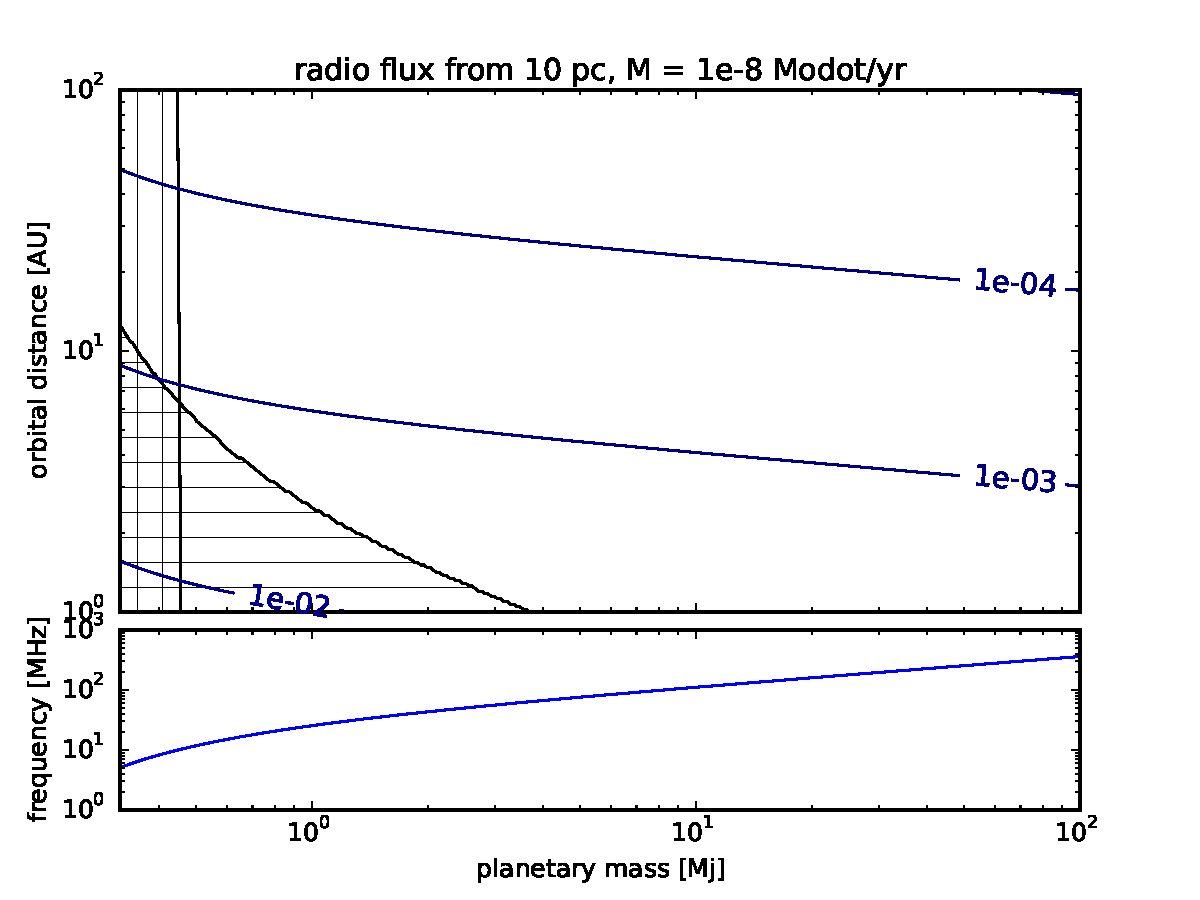
\includegraphics[width=\hsize]{radio_emission_Mdot1e-8_constRp.pdf}
   \plotonesc{radio_emission_Mdot1e-8_constRp_christensen.pdf}
  %\end{center}
 %\end{minipage}
 %\begin{minipage}{0.5\hsize}
   %\begin{center}
   %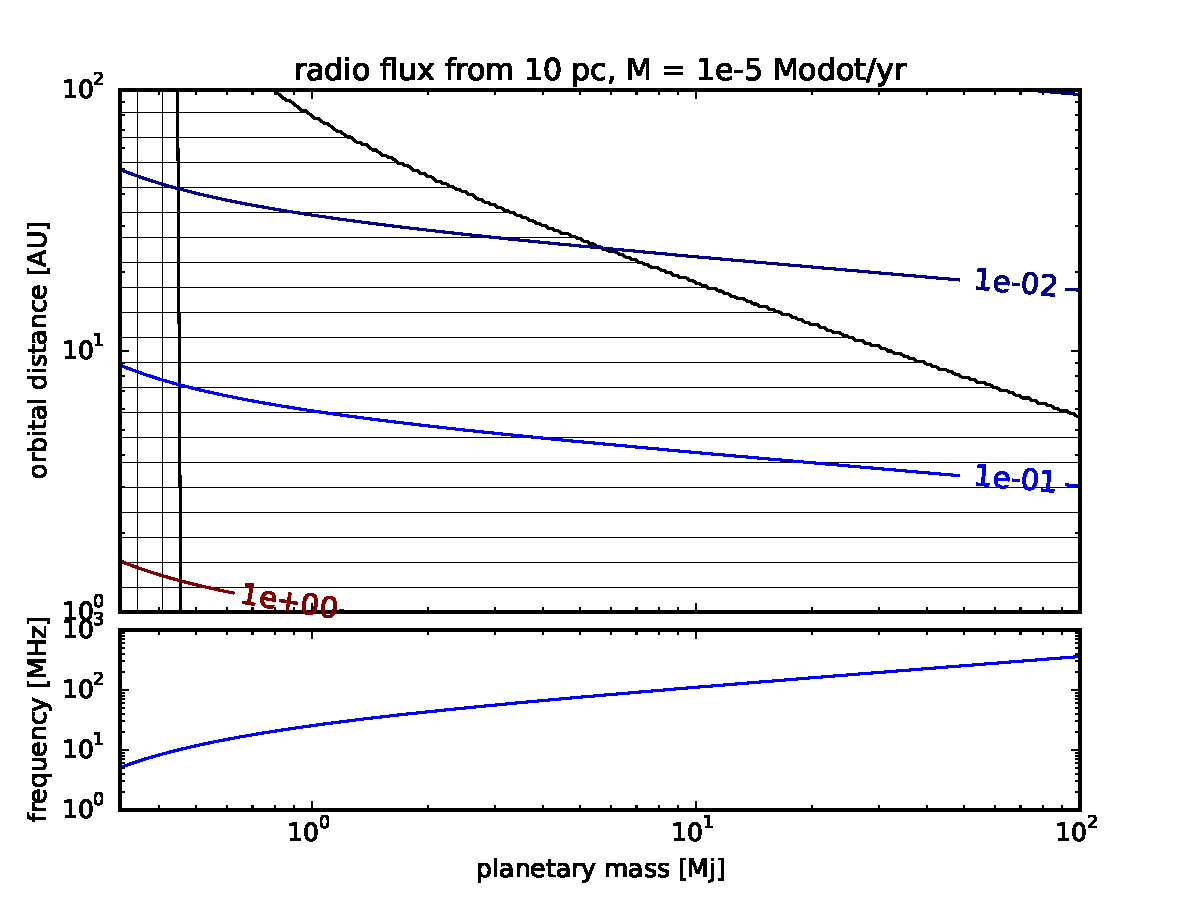
\includegraphics[width=\hsize]{radio_emission_Mdot1e-5_constRp.pdf}
   \plotonesc{radio_emission_Mdot1e-5_constRp_christensen.pdf}
  %\end{center} 
 %\end{minipage}
   \caption{[{\bf New version: based on scaling relationship of Christensen 2010}] Top panel: Intensity of radio emission (in the unit of Jy) from a companion to a RG star (left) and an AGB star at 1 pc. The hashed region with vertical lines are not observable because of the plasma frequency cut-off of Earth's ionosphere. The hashed region with horizontal lines are not observable because of the plasma frequency cut-off of the stellar wind plasma in the vicinity of the companion. Bottom panel: cyclotron frequency, i.e., the frequency of radio emission. }
  \label{fig:radio}
\end{figure*}
%%%%%%%%%%%%%%%%%%%%%%%%%%%%%%%%%%% 



%%%%%%%%%%%%%%%%%%%%%%%%%%%%%%%%%%%
\begin{figure*}[bp]
 %\begin{minipage}{0.5\hsize}
  %\begin{center}
   %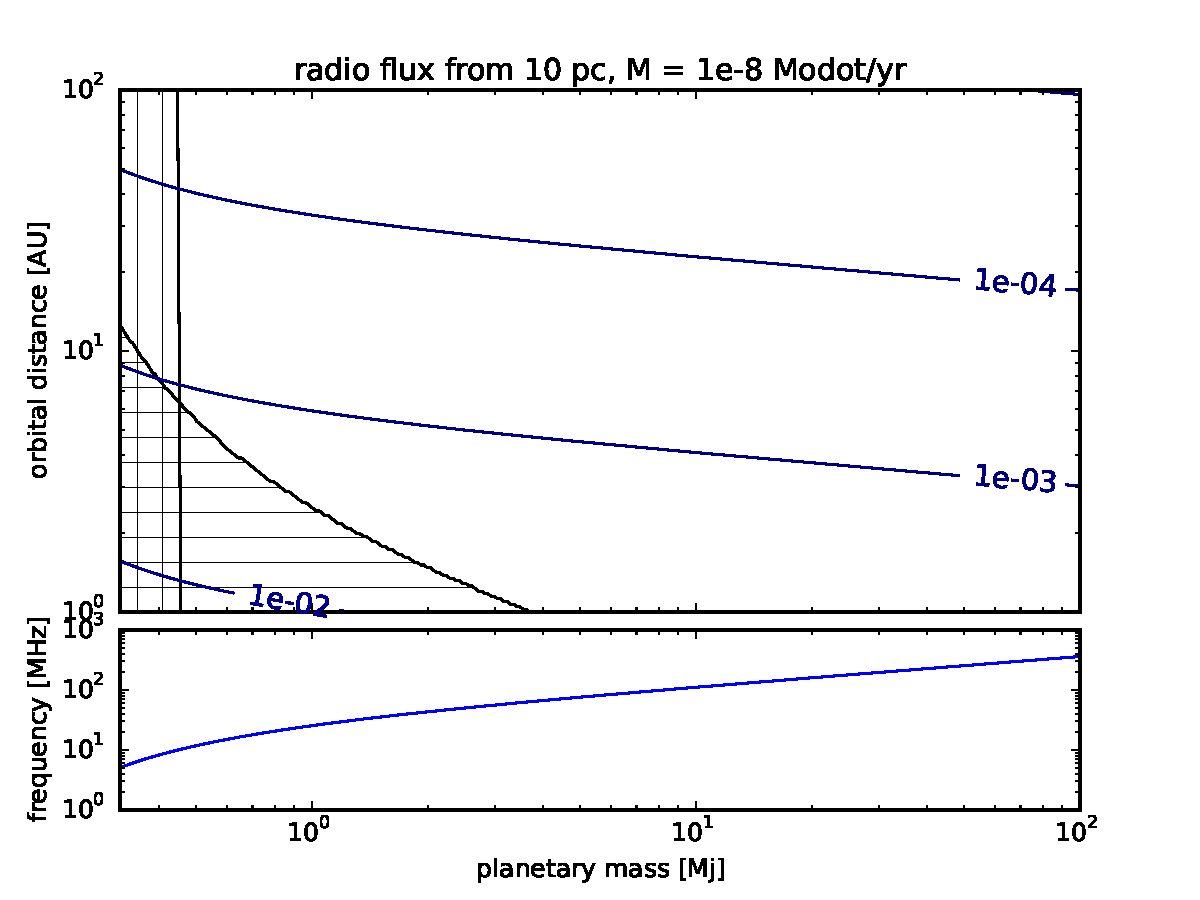
\includegraphics[width=\hsize]{radio_emission_Mdot1e-8_constRp.pdf}
   \plotonesc{radio_emission_Mdot1e-8_constRp.pdf}
  %\end{center}
 %\end{minipage}
 %\begin{minipage}{0.5\hsize}
   %\begin{center}
   %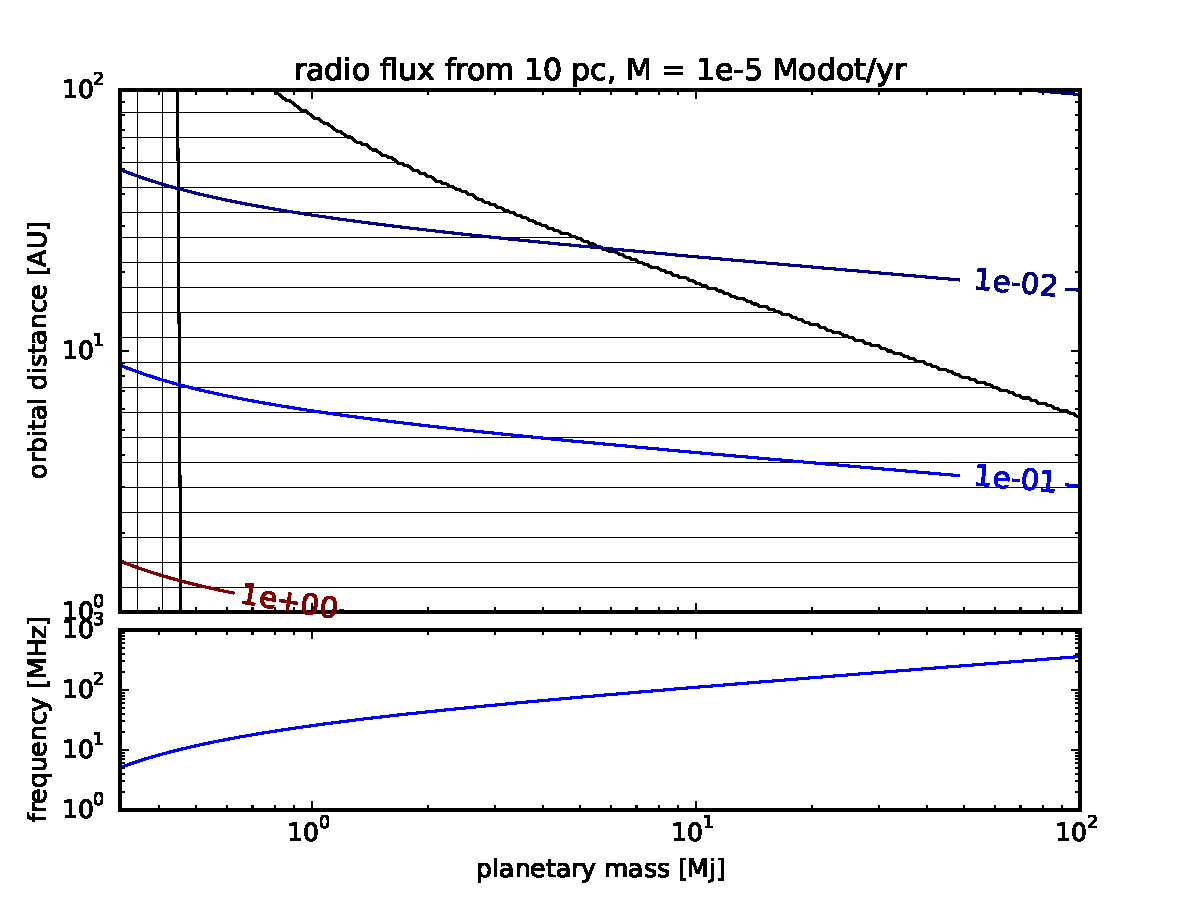
\includegraphics[width=\hsize]{radio_emission_Mdot1e-5_constRp.pdf}
   \plotonesc{radio_emission_Mdot1e-5_constRp.pdf}
  %\end{center} 
 %\end{minipage}
   \caption{[{\bf Old version: based on scaling relationship of Sano 1993}] Top panel: Intensity of radio emission (in the unit of Jy) from a companion to a RG star (left) and an AGB star at 1 pc. The hashed region with vertical lines are not observable because of the plasma frequency cut-off of Earth's ionosphere. The hashed region with horizontal lines are not observable because of the plasma frequency cut-off of the stellar wind plasma in the vicinity of the companion. Bottom panel: cyclotron frequency, i.e., the frequency of radio emission. }
  \label{fig:radio}
\end{figure*}
%%%%%%%%%%%%%%%%%%%%%%%%%%%%%%%%%%%



%%%%%%%%%%%%%%%%%%%%%%%%%%%%%%%%%%%%%%%%%%%%%%%%%%%%%%%%%%%%%%%%%%%%%%%%
\newpage

%%%%%%%%%%%%%%%%%%%%%%%%%%%%%%%%%%%%%%%%%%%%%%%%%%%%%%%%%%%%%%%%%%%
\section{Discussions}
\label{s:discussion}
%%%%%%%%%%%%%%%%%%%%%%%%%%%%%%%%%%%%%%%%%%%%%%%%%%%%%%%%%%%%%%%%%%%

%%%%%%%%%%%%%%%%%%%%%%%%%%%%%%%%%%%%%%%%%%%%%%%%%%%%%%%%%%%%%%%%%%%
\subsection{Intrinsic radio emission of red giants stars}
\label{ss:RGradio}
%%%%%%%%%%%%%%%%%%%%%%%%%%%%%%%%%%%%%%%%%%%%%%%%%%%%%%%%%%%%%%%%%%%

(Jason?)

In the radio range, the brightness source of the radio emission is Rayleigh-Jeans tail of the Planck function, i.e., $S_{\nu } = 2kT\nu^2/c^2$. Recent observations revealed that this dependence on $\nu$ ($f \propto \nu^{\alpha }$ where $\alpha $ is 2) can approximately be extended as low frequency as 1 GHz \citep{gorman2013}, presumably as a result of the wavelength dependence of the opacity (at longer wavelength we see the region further from the center of the stars) and the decreased temperature as the distance from the stars increases. 
In this paper, we simply assume that the radio emission from the red giants themselves is approximated as a black body radiation at 1000~GHz and proportional to $\nu ^2$. 
Thus, the flux from the giants is:
%%%
\begin{eqnarray}
f_{\star } (\nu ) &=& \frac{2R_{\star }^2 k_B T \nu^2}{c^2 d^2}  \\
&\approx & 1.4 \times 10^{-5} ~\mbox{Jy} \left( \frac{d}{10 ~\mbox{pc}} \right)^{-2} \\
&& \times \left( \frac{R_{\star }}{10 R_{\odot }} \right)^2 \left( \frac{T_{\star }}{10^{4}~\mbox{K}} \right) \left( \frac{\nu}{1 ~\mbox{GHz}} \right)^2 
\end{eqnarray}
%%%
The brightest emission due to interaction with planetary companion would overwhelm radio emission from their host (evolved) star in the 10-100~MHz range (in the 100-1000~MHz range) if the stellar radius $R_{\star }$ is smaller than $\sim 1000R_{\odot }$ ($\sim 100R_{\odot }$). 


%%%%%%%%%%%%%%%%%%%%%%%%%%%%%%%%%%%%%%%%%%%%%%%%%%%%%%%%%%%%%%%%%%%
\subsection{Detectability} 
\label{ss:detectability}

Figure \ref{fig:} displays the detection limit of current and near-future radio wave detectors. Between 10~MHz and 100~MHz the detection limit is $\sim 10^{-3}$~Jy. Therefore, Jovian planets around the nearest evolved stars would be within reach. 
On the other hand, between 100~MHz and 1~GHz where the cyclotron frequency of massive Jovian planets resides, SKA potentially achieve $10^{-5}$ Jy. In this range, massive planetary companion as far as 100 pc away would be marginally within the scope. 

We estimate the population of RGHJs within 100 pc to be order of 1000, based on the photometric dataset of Hipparcos. Thus, 


\newpage



%%%%%%%%%%%%%%%%%%%%%%%%%%%%%%%%%%%%%%%%%%%%%%%%%%%%%%%%%%%%%%%%%%%
\subsection{Will the electron spiraling and offset the magnetic field? (Mehrdad Mirababayi)}
\label{ss:offset}


\citet{gorman2013}




%%%%%%%%%%%%%%%%%%%%%%%%%%%%%%%%%%%%%
%\subsection{}

%%%%%%%%%%%%%%%%%%%%%%%%%%%%%%%%%%%%%%%%%%%%%%%%%%%%%%%%%%%%%%%%%%%%%%%%
\section{Conclusions}
\label{sec:conc}

In this paper, we propose that ``hot Jupiters'' around evolved stars (RGHJ) may be bright radio wave emitters, on the assumption of the simple empirical correlation between the radio emission and the kinetic input energy. 
Due to the massive stellar wind, the input kinetic energy into magnetospheres of distant Jovian planets around red giants and AGB stars can be comparable to or by far greater than canonical hot Jupiters in close-in orbits, which could lead to the intrinsic bright radio emission. 

The maximum radio emission we can expect to observe is limited by the plasma cut-off frequency of the stellar wind in the vicinity of the planets. 
For a planet with the same magnetic moment as Jupiter, the maximum radio emission from the planets which can penetrate through the surrounding plasma is $\sim 10^{-3}$ Jy or $\sim 10^{-5}$ Jy at 10 pc and 100 pc, respectively. 
This energy level would be detectable with LWA between 10~MHz abd 100~MHz or with SKA between 100~MHz and 1~GHz. 

The planetary magnetic moment is computed based on the simple scaling relationship given by \citep{christensen2010}. 


The radio emission due to the interaction between the planetary companion and the stellar wind would be brighter than the intrinsic radio emission from the host star. 

The candidate radio detectors sensitive to the radio emission from 10~MHz to 1~GHz are LWA are SKA. For LWA, 

This is above the detection limit of the 

Non-detection 


For planets around AGB stars, be
, which provides us to 


\vspace{0.5in}

%\acknowledgements

{\sc Acknowledgments}

We thank many people for useful discussions, in particular Tony
Mroczkowzki.  YF is supported from the Grant-in-Aid No. 25887024 by the Japan Society for the Promotion of Science. 
DSS gratefully acknowledges support from a fellowship
from the AMIAS group.  NM acknowledges support from [???].

%\newpage

%mehrdad

%\newpage

\bibliography{biblio.bib}


\clearpage

%\end{document}

\section{Dave's sketch}

\citep{spiegel2008}

\citep{lecavelier_et_al2013}

\citep{janhunen_et_al2003}

\citep{zarka1992, zarka1998}

\citep{farrell_et_al2004}

\citep{lazio+farrell2007}: likelihood function, tau Boo search

\citep{lecavelier_et_al2009}

\citep{spiegel2012}

\citep{nordhaus+spiegel2013}



\citep{jiang+jin1996}: 12cm radio of Jupiter during Shoemake-Levy-9

\citep{morin2012, morin_et_al2013}

\citep{christensen_et_al2009, christensen2010}

\citep{saar2001}: Inverse rossby number scaling of magnetic field: $B
\sim 60 {\rm~G} \times Ro^{-1.2}$.  Here, he takes $Ro = \tau_c/P_{\rm
  rot}$, where $\tau_c$ is the convective turnover time = ?
\citep{gilliland1986}.  Well, $F \sim \rho v_c^3 \sim \rho
(H/\tau_c)^3$, so $\tau_c \sim H (\rho / F)^{1/3} = H / (\sigma T_{\rm
  eff}^4 / \rho)^{1/3}$.  Alternatively, $\tau_{\rm conv} \sim (M R^2
/ L)^{1/3}$.

On dimensional grounds, the convective turnover time goes as
$\tau_{\rm conv} \sim (M R^2 / L)^{1/3}$.  According to
\citet{burrows_et_al2001}, radius $R$ and luminosity scale with time
as $R \sim R_J$, where $R_J$ is the radius of Jupiter, and
\begin{equation}
\frac{L}{10^{-9} L_\odot} \sim \left( \frac{t}{1 \rm~Gyr} \right)^{-1.3} \left( \frac{M}{1~M_J} \right)^{2.64} \, .
\label{eq:burrowsLum}
\end{equation}
So,
%\begin{eqnarray}
%\nonumber \tau_{\rm conv} & \sim & 3 {\rm~days} \times \left( \frac{M}{M_J} \right)^{1/3} \left( \frac{R}{R_J} \right)^{2/3} \left( \frac{L}{L_\odot} \right)^{-1/3} \\
% & = & 
%\end{eqnarray}
\begin{eqnarray}
\nonumber \tau_c & \sim & 3 {\rm~hrs} \times \frac{\left( \frac{H}{100 \rm~km} \right) \left( \frac{\rho}{10^{-5} \rm~g~cm^{-3}} \right)^{1/3}}{\left( \frac{L}{10^{-9} L_\odot} \right)^{1/3}} \\
 & = & 3 {\rm~hrs} \times \frac{\left( \frac{H}{100 \rm~km} \right) \left( \frac{\rho}{10^{-5} \rm~g~cm^{-3}} \right)^{1/3}}{\left( \frac{M}{1 ~M_J} \right)^{0.88} \left( \frac{t}{1 \rm~Gyr} \right)^{0.43}} \\
\end{eqnarray}
So the Rossby number $Ro = \tau_c/P_{\rm rot}$ is
\begin{eqnarray}
Ro & = & \frac{\tau_c}{P_{\rm rot}} \\
 & = & \left( \frac{P_{\rm rot}}{3 \rm~hrs} \right)^{-1} \times \frac{\left( \frac{H}{100 \rm~km} \right) \left( \frac{\rho}{10^{-5} \rm~g~cm^{-3}} \right)^{1/3}}{\left( \frac{M}{1 ~M_J} \right)^{0.88} \left( \frac{t}{1 \rm~Gyr} \right)^{0.43}}
\end{eqnarray}

\citep{hallinan_et_al2013}

\citep{desch+kaiser1984} radiometric Bode's law

Noting that
\begin{equation}
\dot{M}_* = 4\pi r^2 \rho[r] v \, ,
\label{eq:mdot
}\end{equation}
so $\rho[r] = \dot{M}_*/(4\pi r^2 v)$,
\begin{eqnarray}
\frac{\rho v^2}{2} = \frac{B^2}{8\pi} \sim \frac{B_0^2}{8\pi} \left( \frac{d}{d_0} \right)^{-3} \, ,
\end{eqnarray}
where $B_0$ is the field strength at a distance $d_0$ from the planet.
\begin{eqnarray}
\frac{\rho v^2}{2} & \sim & \frac{B_0^2}{8\pi} \left( \frac{d}{d_0} \right)^{-6} \\
\frac{\dot{M}_* v}{8\pi a^2} & = & \frac{B_0^2}{8\pi} \left( \frac{d}{d_0} \right)^{-6} \\
\frac{\dot{M}_* v}{r^2} & = & B_0^2 \left( \frac{d}{d_0} \right)^{-6} \\
d^6 & = & \frac{d_0^6 B_0^2 r^2}{\dot{M}_* v} \\
d_A & = & d_0 \left( \frac{B_0^2 r^2}{\dot{M}_* v} \right)^{1/6} \\
  & \sim & 4 R_J \left( \frac{d_0}{R_J}\right) \left\{ \frac{\left( \frac{B}{10 \rm~G} \right)^2 \left( \frac{r}{5 \rm~AU} \right)^2}{\left( \frac{\dot{M}_*}{10^{-6} M_\odot/\rm yr} \right) \left( \frac{v}{20 \rm~km/s} \right)} \right\}^{1/6}
\label{eq:Chapman-Ferraro}
\end{eqnarray}
In the above, $d_A$ is the distance from the planet to the Alfven
point, where the magnetic energy density $u_B = B^2 / 8\pi$ equals the
kinetic energy density in the stellar wind $u_w = \rho v^2/2$, and
$B_0$ is the magnetic field strength at distance $d_0$.

The escape speed is
\begin{equation}
v_{\rm esc}^* = \sqrt{\frac{2 G M_*}{R_*}} \, ,
\end{equation}
so if the stellar wind speed is a factor $C$ times the escape speed, then ...

The power incident on the planet within $d_A$ is
\begin{eqnarray}
P_{\rm inc} & = & \frac{\rho v^3}{2} \times \pi d_A^2 \\
\frac{\rho v^2}{2} & \sim & \frac{B_0^2}{8\pi} \left( \frac{d}{d_0} \right)^{-6} \\
d_A^6 & = & d_0^6 \frac{B_0^2}{4\pi \rho v^2} \\
d_A^2 & = & d_0^2 \left( \frac{B_0^2}{4\pi \rho v^2}\right)^{1/3} \\
\pi d_A^2 \frac{\rho v^3}{2} & = & \frac{d_0^2}{2} \left( \frac{\pi^2 \rho^2 v^7 B_0^2}{4} \right)^{1/3} \\
P_{\rm inc} & = & d_0^2 \left( \frac{\pi^2 \rho^2 v^7 B_0^2}{32} \right)^{1/3} 
%\frac{\dot{M}_* v}{8\pi a^2} & = & \frac{B_0^2}{8\pi} \left( \frac{d}{d_0} \right)^{-6} \\
%\frac{\dot{M}_* v}{r^2} & = & B_0^2 \left( \frac{d}{d_0} \right)^{-6} \\
%d^6 & = & \frac{d_0^6 B_0^2 r^2}{\dot{M}_* v} \\
%d_A & = & d_0 \left( \frac{B_0^2 r^2}{\dot{M}_* v} \right)^{1/6} \\
%  & \sim & 4 d_0 \left\{ \frac{\left( \frac{B}{10 \rm~G} \right)^2 \left( \frac{r}{5 \rm~AU} \right)^2}{\left( \frac{\dot{M}_*}{10^{-6} M_\odot/\rm yr} \right) \left( \frac{v}{20 \rm~km/s} \right)} \right\}^{1/6}
\end{eqnarray}
Note that $\rho v = \dot{M}_*/4\pi r^2$.  Therefore,
\begin{eqnarray}
P_{\rm inc} & = & d_0^2 \left( \frac{\pi^2 \rho^2 v^7 B_0^2}{32} \right)^{1/3} \\
 & = & d_0^2 \left( \frac{\dot{M}_*^2 v^5 B_0^2}{512 r^4} \right)^{1/3} \\
 & = & \frac{d_0^2}{8} \left( \frac{\dot{M}_*^2 v^5 B_0^2}{r^4} \right)^{1/3} \\
\nonumber  & \sim & 2 \times 10^{18} {\rm~W} \left( \frac{d_0}{R_J} \right)^2 \left( \frac{\dot{M}_*}{10^{-5} M_\odot / {\rm yr}} \right)^2 \\
 & & \times \left( \frac{v}{20 \rm~km/s} \right)^5 \left( \frac{B_0}{10 \rm~G} \right)^2 \left( \frac{r}{5 \rm~AU} \right)^{-4}
\end{eqnarray}


The power incident on the planet is

%\citep{lunine_et_al1989} -- error?

% http://kiss.caltech.edu/workshops/magnetic2013/presentations/winterhalter.pdf

%ftp://ftp.iwf.oeaw.ac.at/pub/Scherf/PRE-CD%20V2/pre6/nigl.pdf

%%%%%%%%%%%%%%%%%%%%%%%%%%%%%%%%%%%%%%%%%%%%%%%%%%%%%%%%%%%%%%%%%%%
\subsection{Assumptions for Planetary Magnetic Field}
%\label{ss:magneticfield}
%%%%%%%%%%%%%%%%%%%%%%%%%%%%%%%%%%%%%%%%%%%%%%%%%%%%%%%%%%%%%%%%%%%

\memoYF{It may be better to consider Cristensen's scaling, taking account of the age. But I have not followed the theory yet.}

Theoretically, the magnetic moment of gaseous planets are expressed with the following scaling relationship \citep{griebmeier2004}:
%%%%%%%%%% 
\begin{equation}
\mathcal{M} \propto  \omega ^{\alpha } \rho_c ^{\beta } r_c^{\gamma } \sigma ^{\delta }
\end{equation}
%%%%%%%%%%
where $\omega $ is the spin angular velocity, $\rho _c$, $r_c$ and $\sigma $ are the density, the radius, and the conductivity of the ``dynamo region'' where the density is high enough for hydrogen to be metallic, respectively. 
The scaling indexes are estimated to be $\alpha \sim 1/2-1$, $\beta \sim 1/2$, $\gamma \sim 3-4$, and $\sigma \sim -1/2-0$. In this paper, we assume $\alpha =1$, $\beta =1/2$, and $r_c = 7/2$ \citep{sano1993}. \memoYF{validity?}

Unlike usual hot jupiters, RGHJs are not subject to tidal lock, as the gravitational effects of their host star does not change even if the star evolves into red giants. Without no physical insights of the typical spin rate, we simply assume that of Jupiter: $\omega = 9.925$ [hr]. 
\memoYF{Would their spin rate become higher or lower??}

In order to evaluate $\rho _c $ and $r_c$, we need a model of internal structure of gaseous planets. 
First, we assume that the planetary radius is constant at $R_p = R_{p,J}$, as the numerical calculations show that the radii of gaseous planets over the range of $0.1 R_{p, J} < M_p < 10M_{p, J}$ (with core mass less than 10\%) are converged to $0.8 R_{p, J} < R_p < 1.2R_{p, J}$ in 1 Gyr \citep{fortney2007}. 
For the density profile, we assume a polytrope gas sphere with index $n=1$, which results in:
%%%%%%%%%% 
\begin{equation}
\rho [r] = \left( \frac{\pi M_p}{4 R_p^3} \right) \frac{\sin \left[ \pi \frac{r}{R_p} \right]}{\left( \pi \frac{r}{R_p} \right)}. \label{eq:rho_r}
\end{equation}
%%%%%%%%%%
We determine the core radius $r_c$ by assuming that the hydrogen becomes metallic when $\rho (r)$ exceeds the critical density $\rho_c=700\,\mbox{kg/m}^3$. The density of the metallic core, $\rho _c$ is obtained by averaging the density in the core. 
We assume that the conductivity $\sigma $ is the same as Jupiter \memoYF{?}. 




\end{document}

